% Author: Clara Eleonore Pavillet
% Version: 1.0
% This work is licensed under a Creative Commons Attribution 4.0 International License.

\documentclass[12pt, a4paper]{report}
\input{Packages.tex}
\hypersetup{pdftitle = Thesis, pdfauthor = {First Last}, pdfstartview=FitH, pdfkeywords = essay, pdfpagemode=FullScreen, colorlinks, anchorcolor = red, citecolor = blue, urlcolor=blue, filecolor=green, linkcolor=red, plainpages=false}
%%%%%%%%%%%%%%%%%%%%%%%%%%%%%%%%%%%%%%%%%%%%%%%%%%%%%%%%%%%%%%%%%%%%%%%
\pagestyle{fancy}
\chead{}
\lhead{University of Oxford}
\lfoot{\date{}}
\cfoot{}
\rfoot{\thepage}
% Top and Bottom Line Rules
\renewcommand{\headrulewidth}{0.4pt} %0.4pt
\renewcommand{\footrulewidth}{0.4pt}
\fancyheadoffset{9pt}
\fancyfootoffset{9pt}
% Line spacing
\renewcommand{\baselinestretch}{1.5} %1.5
%%%%%%%%%%%%%%%%%%%%%%%%%%%%%%%%%%%%%%%%%%%%%%%%%%%%%%%%%%%%%%%%%%%%%%%
\date{}

\title{Random Title on Mathematical and Computational Modelling}
\author{\\ \Large{Wonsuk Yang}
\\
\\
\\ Candidate Number: 000000
\\
\\ University of Oxford
\\
A dissertation submitted for the degree of \\ \textit{Master of Science}
\\ \\
Trinity 2022
\\ \small{Word Count: 0000}
}
%%%%%%%%%%%%%%%%%%%%%%%%%%%%%%%%%%%%%%%%%%%%%%%%%%%%%%%%%%%%%%%%%%%%%%%
\begin{document}
% Adjust logo positions here
\AddToShipoutPicture*{\BackgroundPicturea{Logos/logo2.png}{0.7in}{5.8in}}
\thispagestyle{headings}
	\maketitle
\FloatBarrier
\pagenumbering{roman}

\thispagestyle{empty}
\begin{abstract}
\lipsum[1-2]

\keywords{Keyword1 - Keyword2 - Keyword3}
% \vspace{-10mm} %To remove added white space after
\end{abstract}
\tableofcontents
% \thispagestyle{plain}
% \listoffigures
% \listoftables

% \chapter*{List of Abbreviations}
% \begin{abbreviations}
%     \item[MAS] Multi-Agent System
% \end{abbreviations}

\chapter{Introduction}
\pagenumbering{arabic}
\section{Motivation}
\lipsum[1-3]
\section{Aim and Objectives}
\lipsum[6]
\section{Thesis Outline}
The remainder of this report is organised as follows:
\begin{itemize}
    \item[] \textbf{Chapter} \hyperref[Chap2]{\textbf{2}} --- introduces ...
    \item[] \textbf{Chapter} \hyperref[Chap3]{\textbf{3}} --- ...
    \item[] \textbf{Chapter} \hyperref[Chap4]{\textbf{4}} --- ...
\end{itemize}
\chapter{Methodology}
\label{Chap2}
We can cite an article as an example \cite{DeepMindRef}. \lipsum[4-8]
\begin{table}[H]
   \caption{Example Table}
   \small
   \centering
   \begin{tabular}{lccccr}
   \toprule[\heavyrulewidth]\toprule[\heavyrulewidth]
   \textbf{C1} & \textbf{C2} & \textbf{C3} & \textbf{C4}\\ 
   \midrule
\multirow{3}{*}{\textbf{Row}}& Val & Val & \textcolor{igreen}{GreenVal}\\
   & & Val  & \textcolor{igreen}{Val}\\
& &  & \textcolor{igreen}{Example}\\ \hdashline
   \bottomrule[\heavyrulewidth] 
   \end{tabular}
\end{table}


\chapter{Results}
\label{Chap3}
\lipsum[1-4]
\begin{figure}
    \centering
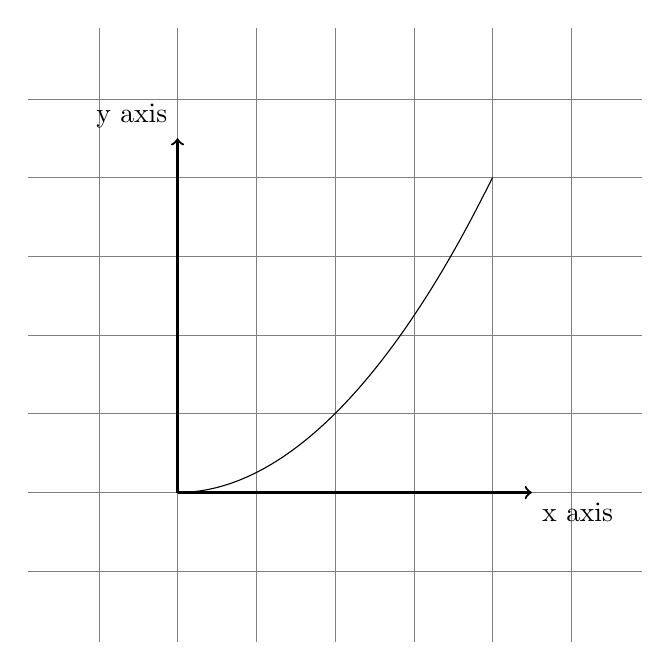
\begin{tikzpicture}
    \draw[step=1cm,gray,very thin] (-1.9,-1.9) grid (5.9,5.9);
    \draw[thick,->] (0,0) -- (4.5,0) node[anchor=north west] {x axis};
    \draw[thick,->] (0,0) -- (0,4.5) node[anchor=south east] {y axis};
    \draw (0,0) parabola (4,4);
\end{tikzpicture}
\caption{Example TikZ Figure}
\end{figure}
\chapter{Discussion}
\label{Chap4}
\lipsum[9-10]

\renewcommand{\bibname}{Bibliography}
\bibliographystyle{apacite}
\bibliography{Bibliography.bib}

\begin{appendices}
\chapter{Appendix Example}
\end{appendices}

\end{document}